\documentclass[../main.tex]{subfiles}
\LoadClass[a4paper,12pt]{article}
\documentclass{article}

%%%%%%%%%%%%%%%%%%%%%%%%%%%%%%%
%     import des packages     %
%%%%%%%%%%%%%%%%%%%%%%%%%%%%%%%
\usepackage[export]{adjustbox}
\usepackage{algorithm}
\usepackage{algorithmic}
\usepackage{amsmath,amsfonts,amssymb}
\usepackage{anyfontsize}
\usepackage{array}
\usepackage[english]{babel}
\usepackage{colortbl}
\usepackage{comment}
\usepackage{cclicenses}
\usepackage{eqnarray}
\usepackage{eso-pic}
\usepackage{dirtree}
\usepackage{fancybox}
\usepackage{fancyhdr}
\usepackage{float}
\usepackage[T1]{fontenc} 
\usepackage{forest}
\usepackage{fourier-orns}
\usepackage{gensymb}
\usepackage{geometry}
\usepackage{glossaries}
\usepackage{graphicx}
\usepackage{hyperref}
\usepackage{ifthen}
\usepackage{import}
\usepackage{indentfirst}
\usepackage[utf8]{inputenc}
\usepackage{lastpage}
\usepackage{libertine}
\usepackage{lipsum}
\usepackage{listings}
\usepackage{mathtools}
\usepackage{mdframed}
\usepackage{multicol}
\usepackage{pdfpages}
\usepackage{pifont}
\usepackage{stmaryrd}
\usepackage{subcaption}
\usepackage{subfiles}
\usepackage{tabularx}
% \usepackage{tcolorbox}
\usepackage[most]{tcolorbox}
\usepackage{textcomp}
\usepackage{ulem}
\usepackage{wrapfig}

%%%%%%%%%%%%%%%%%%%%%%%%%%%%%%%%%%%%%%%%%%%%%%%%%%%%%%%%%
%    Renseigner les titres et variables importantes     %
%%%%%%%%%%%%%%%%%%%%%%%%%%%%%%%%%%%%%%%%%%%%%%%%%%%%%%%%%
\newcommand{\titre}{Multi-robot coordination}
\newcommand{\soustitre}{Autonomous exploration of gallery networks}
\newcommand{\sujet}{Engineering Graduation Project}
\newcommand{\sujets}{Seatech 3A - MOCA}
\newcommand{\auteur}{Fabien MATHÉ}
\newcommand{\referent}{M. Mehmet ERSOY}
\newcommand{\reportdate}{\date}

\newcommand{\partA}{State of the art}
\newcommand{\partB}{Partie 2}
\newcommand{\partC}{Partie 3}
\newcommand{\partD}{Partie 4}
\newcommand{\partE}{Partie 5}

%%%%%%%%%%%%%%%%%%%
%     BOOLEEN     %
%%%%%%%%%%%%%%%%%%%

% Création des boolean
\newboolean{abst}
\newboolean{thx}
\newboolean{contents}
\newboolean{introduction}
\newboolean{pt2}
\newboolean{pt3}
\newboolean{pt4}
\newboolean{pt5}
\newboolean{conclusion}
\newboolean{perspectives}
\newboolean{glossaire}
\newboolean{biblio}
\newboolean{annexe}


% Renseigner si le Rapport contient un abstract
\setboolean{abst}{true}
% Renseigner si le Rapport contient des remerciements
\setboolean{thx}{true}
% Renseigner si le Rapport contient une table des matières
\setboolean{contents}{true}
% Renseigner si le Rapport contient une introduction
\setboolean{introduction}{true}
% Renseigner si le Rapport contient une partie 2
\setboolean{pt2}{true}
% Renseigner si le Rapport contient une partie 3
\setboolean{pt3}{true}
% Renseigner si le Rapport contient une partie 4
\setboolean{pt4}{true}
% Renseigner si le Rapport contient une partie 5
\setboolean{pt5}{true}
% Renseigner si le Rapport contient une introduction
\setboolean{conclusion}{true}
% Renseigner si le Rapport contient des perspectives
\setboolean{perspectives}{true}
% Renseigner si le document contient une bibliographie
\setboolean{biblio}{true} 
% Renseigner si le document contient un glossaire
\setboolean{glossaire}{false}
% Renseigner si le Rapport contient des annexes 
\setboolean{annexe}{true}


%%%%%%%%%%%%%%%%%%%%%%%%%%%%%%%%%%%%%%
%     En-têtes en pieds de pages     %
%%%%%%%%%%%%%%%%%%%%%%%%%%%%%%%%%%%%%%
\geometry{hmargin=2cm,vmargin=2.3cm}
\pagestyle{fancy}
\fancyhfoffset[]{0pt}
\setlength{\headheight}{28pt}
\lhead{
\includegraphics[height = 0.6cm]{IMAGES/logos/Logo_SeaTech_2023.png}}
% \rhead{
\includegraphics[height = 0.7cm]{IMAGES/logos/MOCA.png}}
\rhead{\textsc{\leftmark}}

% Update \rightmark with \section name
\renewcommand{\sectionmark}[1]{\markboth{#1}{#1}}


\lfoot{\auteur}
\cfoot{ }
\rfoot{Page \thepage \ / \pageref{LastPage}}

\title{\titre}
\author{\auteur}
\date{\today}

%%%%%%%%%%%%%%%%%%%%%%%%%%%%%%
%     Autre mise en page     %
%%%%%%%%%%%%%%%%%%%%%%%%%%%%%%
\numberwithin{figure}{section}
\numberwithin{table}{section}

\setcounter{tocdepth}{2} % Change to 1 to exclude subsections as well


\newcommand{\citeURL}[1]{\href{#1}{\detokenize{#1}}}

% Création du compteur d'annexes
\newcounter{annexecounter}

% Définition de la commande pour les annexes
\NewDocumentCommand{\annexe}{m}{%
    \stepcounter{annexecounter} % Incrémenter le compteur d'annexes
    \subsection*{Annexe \arabic{annexecounter} - #1} % Affichage du texte avec le numéro et le titre
	\label{sec:#1}
}

\newcommand{\tobedone}{\textcolor{red}{\LARGE \textbf{TO BE DONE}}}
\newcommand{\annexetonum}{\textcolor{red}{\LARGE \textbf{ANNEXE ...}}}

\renewcommand{\familydefault}{\sfdefault}



%%%%%%%%%%%%%%%%%%%%%%%%%%%%%%%%%
%     Mise en page des codes    %
%%%%%%%%%%%%%%%%%%%%%%%%%%%%%%%%%
\definecolor{codegreen}{rgb}{0,0.6,0}
\definecolor{codegray}{rgb}{0.5,0.5,0.5}
\definecolor{codepurple}{rgb}{0.58,0,0.82}
\definecolor{backcolour}{rgb}{0.95,0.95,0.92}

\lstdefinestyle{python}{
	backgroundcolor=\color{backcolour},
	commentstyle=\color{codegreen},
	keywordstyle=\color{blue},
	numberstyle=\tiny\color{codegray},
	stringstyle=\color{codepurple},
	basicstyle=\ttfamily\scriptsize,
	breakatwhitespace=false,
	breaklines=true,
	captionpos=b,
	keepspaces=true,
	numbers=left,
	numbersep=5pt,
	showspaces=false,
	showstringspaces=false,
	showtabs=false,
	tabsize=2
}

\lstset{style=python}
\definecolor{codegreen}{rgb}{0,0.6,0}
\definecolor{codegray}{rgb}{0.5,0.5,0.5}
\definecolor{codepurple}{rgb}{0.58,0,0.82}
\definecolor{backcolour}{rgb}{0.95,0.95,0.92}

\lstdefinestyle{cpp}{
	backgroundcolor=\color{backcolour},
	commentstyle=\color{codegreen},
	keywordstyle=\color{blue},
	numberstyle=\tiny\color{codegray},
	stringstyle=\color{codepurple},
	basicstyle=\ttfamily\scriptsize,
	breakatwhitespace=false,
	breaklines=true,
	captionpos=b,
	keepspaces=true,
	numbers=left,
	numbersep=5pt,
	showspaces=false,
	showstringspaces=false,
	showtabs=false,
	tabsize=2,
	language=C++
}

\lstset{style=cpp}

\definecolor{codegreen}{rgb}{0,0.6,0}
\definecolor{codegray}{rgb}{0.5,0.5,0.5}
\definecolor{codepurple}{rgb}{0.58,0,0.82}
\definecolor{backcolour}{rgb}{0.95,0.95,0.92}

\lstdefinestyle{fortran}{
    backgroundcolor=\color{backcolour},
    commentstyle=\color{codegreen},
    keywordstyle=\color{blue},
    numberstyle=\tiny\color{codegray},
    stringstyle=\color{codepurple},
    basicstyle=\ttfamily\scriptsize,
    breakatwhitespace=false,
    breaklines=true,
    captionpos=b,
    keepspaces=true,
    numbers=left,
    numbersep=5pt,
    showspaces=false,
    showstringspaces=false,
    showtabs=false,
    tabsize=2,
    language=[90]Fortran
}

\lstset{style=fortran}


%%%%%%%%%%%%%%%%%%%%%%%%%%%%%%%%%%%%%%%%%%%%%%%%%%%%%%%%%%%%%%%%%%%%%%%%%%%%%%%%%%%%%%%%%%%%%%%%%%%%%%%%%%%%%%%%%%%%%%%
%                                                  Début du document                                                  %
%%%%%%%%%%%%%%%%%%%%%%%%%%%%%%%%%%%%%%%%%%%%%%%%%%%%%%%%%%%%%%%%%%%%%%%%%%%%%%%%%%%%%%%%%%%%%%%%%%%%%%%%%%%%%%%%%%%%%%%

\begin{document}

%%%%%%%%%%%%%%%%%%%%%%%%%
%     Page de garde     %
%%%%%%%%%%%%%%%%%%%%%%%%%
\begin{titlepage}
	\AddToShipoutPictureBG*{
\includegraphics[width=\paperwidth,height=\paperheight]{IMAGES/PageDeGardeRapport.png}}
	\begin{figure}[H]
		\begin{subfigure}{0.45\linewidth}
				
\includegraphics[width=0.6\textwidth,left]{IMAGES/logos/Logo_SeaTech_2023.png}
		\end{subfigure}
		\hfill
		\begin{subfigure}{0.45\linewidth}
				% 
\includegraphics[width=0.6\textwidth,right]{IMAGES/logos/MOCA.png}
		\end{subfigure}
	\end{figure}

	\centering

	% Espacement vertical
	\vspace*{5cm}

	% Barres horizontales
	\makebox[0.7\linewidth]{\hrulefill}\\[0.2cm]

	% Titre encadré
	\vspace{0.5cm}
	\begin{minipage}{\textwidth}
		\centering
		{\fontsize{28}{48}\selectfont \textsc{\titre}}\\[0.2cm]

		{\fontsize{18}{48}\selectfont \textsc{\soustitre}}
	\end{minipage}
	\vspace{0.3cm}

	% Barres horizontales
	\makebox[0.8\linewidth]{\hrulefill}\\[0.2cm]

	% Espacement vertical
	\vspace{3cm}

	% Description
		\large{\Large \textbf{\sujet}}\\
		\large{\textbf{\sujets}}\\

		\vspace{0.5cm}
		\large{\textbf{\reportdate}}

	\vspace{2cm}

	\begin{minipage}{0.20\textwidth}

	\end{minipage}
	\hfill
	\begin{minipage}{0.35\textwidth}
		\begin{flushleft}
			Auteur : \\
			\auteur
		\end{flushleft}
	\end{minipage}
	\begin{minipage}{0.09\textwidth}
		% Section vide pour espacement optimal
	\end{minipage}
	\hfill
 	\begin{minipage}{0.3\textwidth}
		\begin{flushleft}
			Enseignant : \\
			\referent

		\end{flushleft}
	\end{minipage}


\end{titlepage}

\ClearShipoutPictureBG

\newpage

\renewcommand{\thepage}{}

\renewcommand{\thepage}{\arabic{page}}
\renewcommand{\thesection}{\Roman{section}}

%%%%%%%%%%%%%%%%%%
%     Résumé     %
%%%%%%%%%%%%%%%%%%
\ifthenelse{\boolean{abst}}{
	\addcontentsline{toc}{section}{\protect\numberline{}Résumé}%
	\subfile{SECTIONS/1resume}

	\newpage
}

%%%%%%%%%%%%%%%%%%%%%%%%%
%     Remerciements     %
%%%%%%%%%%%%%%%%%%%%%%%%%
\ifthenelse{\boolean{thx}}{
	\addcontentsline{toc}{section}{\protect\numberline{}Remerciements}%
	\subfile{SECTIONS/2remerciements}

	\newpage
}

%%%%%%%%%%%%%%%%%%%%%%%%%%%%
%     Plan du document     %
%%%%%%%%%%%%%%%%%%%%%%%%%%%%

\ifthenelse{\boolean{contents}}{
	\vfill
	\tableofcontents
	\vfill
	
	\newpage
}

%%%%%%%%%%%%%%%%%%%%%%%%
%     INTRODUCTION     %
%%%%%%%%%%%%%%%%%%%%%%%%
\ifthenelse{\boolean{introduction}}
{
	\addcontentsline{toc}{section}{\protect\numberline{}Introduction}%
	\section*{Introduction}

	\markboth{Introduction}{Introduction} % Manually update \rightmark for section*
	\subfile{SECTIONS/3introduction}


	\newpage
}


%%% PARTIE 1 %%%
\section{\partA}
\subfile{SECTIONS/part1}

%%% PARTIE 2 %%%
\newpage
\ifthenelse{\boolean{pt2}}
{
	\section{\partB}
	\subfile{SECTIONS/part2}
	
	\newpage
}
	
	
%%% PARTIE 3 %%%
\ifthenelse{\boolean{pt3}}
{
	\section{\partC}
	\subfile{SECTIONS/part3}
	
	\newpage
}
	
	
%%% PARTIE 4 %%%
\ifthenelse{\boolean{pt4}}
{
	\section{\partD}
	\subfile{SECTIONS/part4}
	
	\newpage
}
	
%%% PARTIE 5 %%%
\ifthenelse{\boolean{pt5}}{
	\section{\partE}
	\subfile{SECTIONS/part5}

	\newpage
}
		
%%%%%%%%%%%%%%%%%%%%%%
%     CONCLUSION     %
%%%%%%%%%%%%%%%%%%%%%%
\ifthenelse{\boolean{perspectives}}
{
	\addcontentsline{toc}{section}{\protect\numberline{}Conclusion}%
	\section*{Conclusion}
	\markboth{Introduction}{Introduction} % Manually update \rightmark for section*

	\subfile{SECTIONS/Wconclusion}

	\newpage
}



\ifthenelse{\boolean{perspectives}}
{
	\section*{Perspectives}
	\addcontentsline{toc}{section}{\protect\numberline{}Perspectives}
	\subfile{SECTIONS/Xperspectives}
	
	\newpage 
}

%%%%%%%%%%%%%%%%%%%%%%%%%
%     Bibliographie     %
%%%%%%%%%%%%%%%%%%%%%%%%%

\ifthenelse{\boolean{biblio}}
{
	\addcontentsline{toc}{section}{\protect\numberline{}References}
	% \bibliographystyle{unsrt}
	\bibliographystyle{IEEEtran}
	\footnotesize{\bibliography{BIBLIOGRAPHY/bib.bib}}

	\newpage
}


%%%%%%%%%%%%%%%%%%%%%
%     Glossaire     %
%%%%%%%%%%%%%%%%%%%%%
\normalsize
\ifthenelse{\boolean{glossaire}}
{
	\section*{Glossaire}
	\makeglossaries
	\printglossaries
	\addcontentsline{toc}{section}{\protect\numberline{}Glossaire}%
	\subfile{SECTIONS/Yglossaire}
	
	\newpage
}

%%%%%%%%%%%%%%%%%%%
%     Annexes     %
%%%%%%%%%%%%%%%%%%%
\ifthenelse{\boolean{annexe}}
{
	\section*{Annexes}
	\addcontentsline{toc}{section}{\protect\numberline{}Annexes}%
	\subfile{SECTIONS/Zannexes}
}


\end{document}


\begin{document}

\subsection{Global path theory}
In this section, we consider the theoretical path that the robot should follow in a space with obstacles, without taking into account the feasibility constraints imposed by the robot's physical limitations. This theoretical path is derived based on the shortest distance to the target while avoiding obstacles.

Soit $\Omega \in \mathbb{R}^{2}$, soit $\mathbf{X}(t)$ les coordonées du robot à l'instant $t$ dans cet espace.


Soit $ V(t)$ le champ de vision du robot à l'instant $t$

Soit $\mathbf{M}(t, \theta)$ le premier point d'intersection entre un segment et les murs, 

\begin{equation*}
    \displaystyle
    \mathbf{M}(t, \theta) = \mathbf{X}(t) + R(t, \theta) 
    \begin{pmatrix}
        \cos \theta & 0\\
        0 & \sin \theta\\
    \end{pmatrix} 
    \mathbf{X}(t)
\end{equation*}

On note $\mathbf{M}_{max} (t, \theta)$ le point tel que $R(t, \theta) = R_{max}$

Ici,
\begin{equation*}
    \displaystyle
    R(t, \theta) = \min (\text{\rmfamily distance}( \, \mathbf{X}(t), \, L(\theta) \cap W \,))
\end{equation*}

\begin{equation*}
    \displaystyle
    L(\theta) = \left\{ \, (1 - l) \, \mathbf{X}(t) + l\, \mathbf{M}_{max}(t, \theta) \,|\, l \in [0, 1]\, \right\}
\end{equation*}

\begin{equation*}
    \displaystyle
    W = \left\{ \, \text{\rmfamily Segment} (\Omega)\, \right\}
\end{equation*}

On défini le champ de vision du robot tel que:


\begin{equation}
    \displaystyle
    V(t) = \left\{ \, (1 - l) \, \mathbf{X}(t) + l\, \mathbf{M}(t, \theta) \,|\, l \in [0, 1], \theta \in [0, 2 \pi[ \, \right\}
\end{equation}

Autrement dis, $V(t)$ est l'ensemble des points de $\Omega$ présents dans un disque de rayon $R_{max}$ et situé entre le robot et la plus proche intersection à un mur 

On construit maintenant la fonctionnelle que l'on cherchera plus tard à optimiser, celle-ci est relative au déplacement du robot.


On défini $\mathit{KM}$ (\textit{Known Map}) l'espace de la map connu par le robot et $\mathit{EM}$ (\textit{Explorable Map}) la partie de $\Omega$ explorable par le robot.
\begin{equation}
    \displaystyle
    J(\mathbf{X}(t)) = \int_{0}^{T} | \mathbf{\dot{X}}(t) | dt
\end{equation}

$J$ est une fonctionnelle fonction de la position initiale du robot, elle donne la longeur du chamin parcourue par le robot avant que $t = T$.

$T$ étant l'instant à partir du quel la map est explorée au maximum des capacités du robot, c'est à dire : $KM = EM$.

Pour savoir si $KM = EM$, on calcul les contours du domaine connu, si tous les contours sont fermés, alors $KM \subset EM$, si de plus les mesures de $KM$ et de $EM$, à savoir leur surface, sont égales alors, on peut raisonnablement dire que $KM = EM$.


Pour plus de simplicité lors de l'étude de la fonctionnelle, on la modifie légerement.
\begin{equation}
    \displaystyle
    J(\mathbf{X}(t)) = \frac{1}{2} \int_{0}^{T} \mathbf{\dot{X}}(t)^{2} dt
\end{equation}

\subsection{Local path theory}

In this section, we focus on determining the optimal commands for navigating to a local waypoint obstacle-free while adhering to the robot's constraints.

Here, we focus on the energy of the robot to compute the optimal command, If we consider the robot to move using dc motors, the power used by the robot is proportional to the voltage for the rotation speed and the current for the torque applied to the wheel. We consider too that the floor is completely flat and the torque is constant so that the current is always the same. The energy is only related to the wheel speed then we define the Energy spent for moving as :

as a reminder, $\omega_L$ and $\omega_R$ are the speed of the left and right wheel.

$$
\displaystyle E(T) = \int_{0}^{T} \| \omega(t) \| \, dt
$$

with $\displaystyle \| \omega (t) \| = \sqrt{\omega_L^{2}(t) + \omega_R^{2}(t)}$ and  $\omega_{L, R} \,:\, \mathbb{R}_+ \longrightarrow [-\omega_{max}, \omega_{max}]$ 

Two constraint remains, we want $X(0) = X_R$ and $X(T) = X_{WP}$

In the part \figtonum, we calculated $\dot{X} = F(\omega)$.


\subsection{Introducing a new method for dynamic pathfinding}

In this section, we introduce a new method for real-time dynamic pathfinding. This method involves inflating the path perpendicular to the shortest path to a point, i.e., a line. The line is split if it is not free from obstacles within a given safe range.

The principle is simple: draw a straight line between the robot and the waypoint (\autoref{fig:draw_line}). If the path is not free of obstacles within the defined safe range (\autoref{fig:check_line}), split the path in the middle and shoot points perpendicular to the line (\autoref{fig:shoot_line}). When a shot point is free from obstacles, validate the point and check if the two resulting lines are free from obstacles (\autoref{fig:validate_point}). If not, repeat the steps described above on the new lines (\autoref{fig:repeat_method}). Once all points are safe, simplify the path using a straightforward algorithm. The process can be visualized on \autoref{fig:method_visu}.

\begin{figure}[H]
	\centering
	\begin{subfigure}[b]{0.45\textwidth}
		\centering
		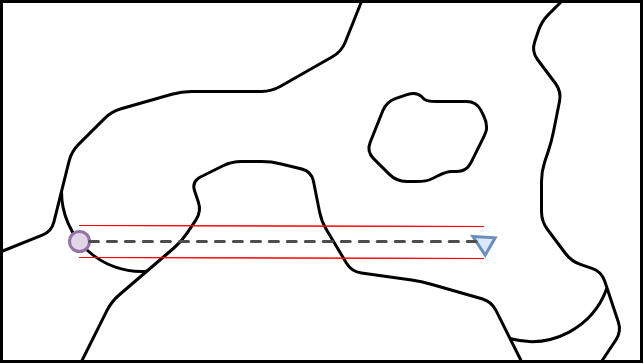
\includegraphics[width=\textwidth]{IMAGES/part3/methode1.png}
		\caption{Draw a straight line}
		\label{fig:draw_line}
	\end{subfigure}
	\hfill
	\begin{subfigure}[b]{0.45\textwidth}
		\centering
		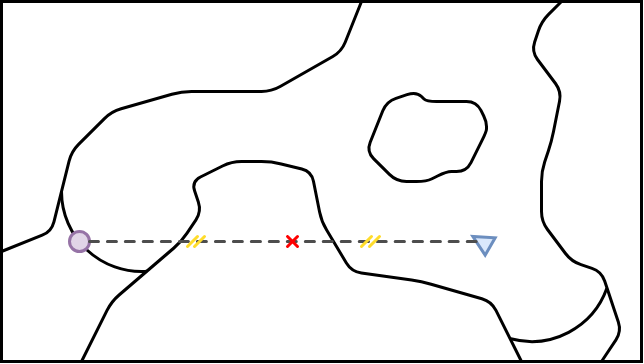
\includegraphics[width=\textwidth]{IMAGES/part3/methode2.png}
		\caption{Check if the path is free}
		\label{fig:check_line}
	\end{subfigure}
	\vfill
	\begin{subfigure}[b]{0.45\textwidth}
		\centering
		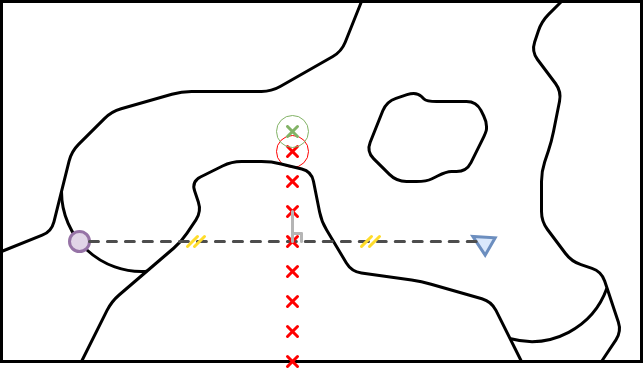
\includegraphics[width=\textwidth]{IMAGES/part3/methode3.png}
		\caption{Shoot points perpendicular}
		\label{fig:shoot_line}
	\end{subfigure}
	\hfill
	\begin{subfigure}[b]{0.45\textwidth}
		\centering
		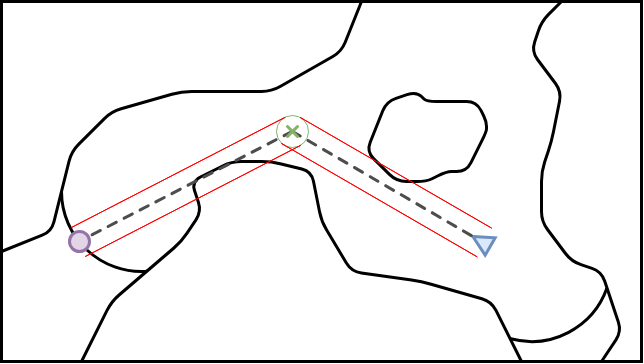
\includegraphics[width=\textwidth]{IMAGES/part3/methode4.png}
		\caption{Validate the point}
		\label{fig:validate_point}
	\end{subfigure}
	\vfill
	\begin{subfigure}[b]{0.45\textwidth}
		\centering
		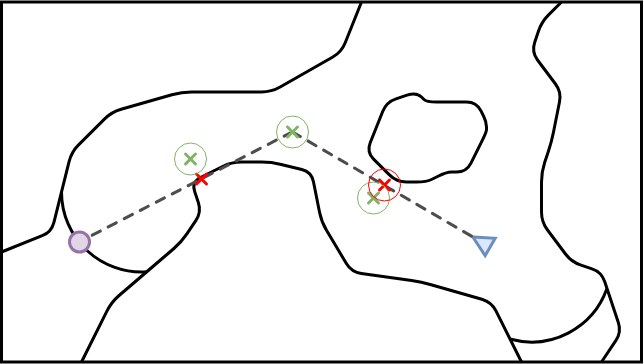
\includegraphics[width=\textwidth]{IMAGES/part3/methode5.png}
		\caption{Repeat the method}
		\label{fig:repeat_method}
	\end{subfigure}
	\hfill
	\begin{subfigure}[b]{0.45\textwidth}
		\centering
		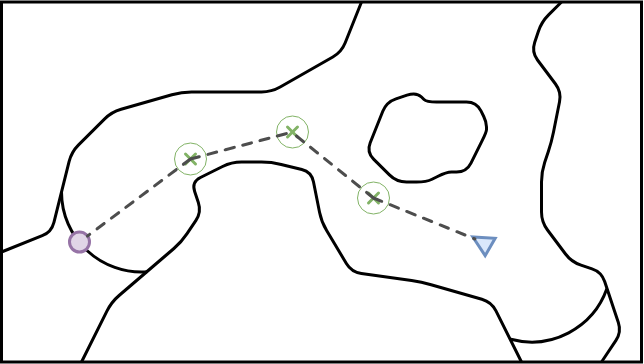
\includegraphics[width=\textwidth]{IMAGES/part3/methode6.png}
		\caption{Simplify the path}
		\label{fig:idk}
	\end{subfigure}
	\caption{Visualization of the dynamic pathfinding method}
	\label{fig:method_visu}
\end{figure}



\textbf{Path simplification}

The goal of this algorithm is to ensure that the path is the shortest possible by simplifying it. The algorithm iterates through all the points in the path. For each point, it checks if the path to the next point is obstacle-free. If it is, the algorithm continues to the next point. If the path is not free, the algorithm keeps the last valid point and starts the process again from there. This way, the path is simplified by removing unnecessary intermediate points while ensuring it remains obstacle-free. The method can be visualized on the \autoref{fig:path_simp}.

\begin{figure}[H]
	\centering
	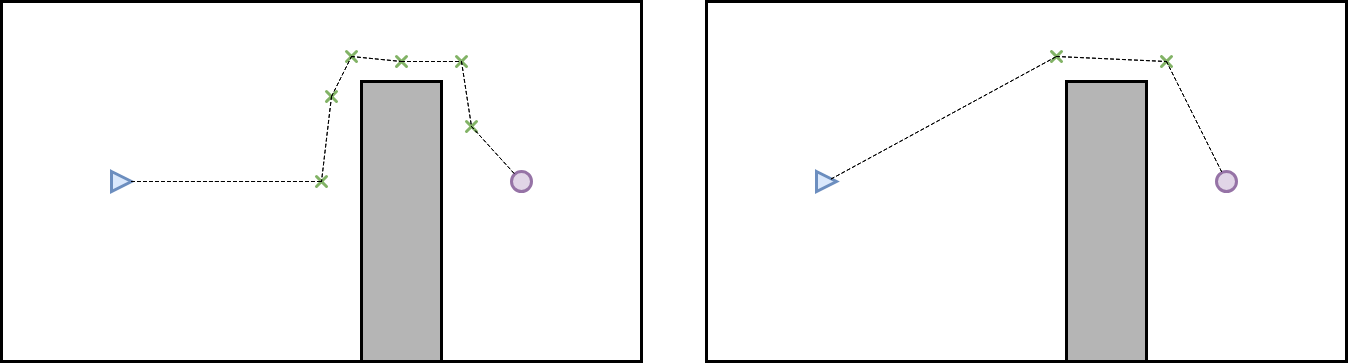
\includegraphics[width=0.9\textwidth]{IMAGES/part3/shorten_path.png}
	\caption{Path simplification process}
	\label{fig:path_simp}
\end{figure}

To ensure this algorithm works and to measure its performance, I conducted a small benchmark. While the benchmark can be theoretically calculated, I also explored a numerical method for computing the shortest path to handle various scenarios. The benchmark will serve as a performance estimator for the numerical method.

\subsection{Finding the shorthest path distance}
To find the shortest path, I like to take inspiration from nature by simulating a wave propagating through a medium. This way, the shortest path naturally emerges as the one the wave follows.  

\vspace{1em}

The wave equation describes how information spreads at a certain speed, but challenges arise—how to model refraction, how to ensure the wave propagates at a constant speed. To tackle this, I used a cellular automaton once again. Made for propagating information, they are an interesting tool for this approach.\cite{tapia_2016}

\vspace{1em}

Differently from the part \figtonum, I will use cellular automata as a computational tool for simulating phenomenon. Application were found in various domain from physics to biology. Lattice Gaz Cellular Automata (LGCA) for instance are used to simulate gaz fluid flows, it is the precursor of the lattice Boltzman Method (LBM)\cite{chen_1998}

\vspace{1em}

Based on the work of \textit{Calvo Tavia} and \textit{al.}\cite{tapia_2016}, the process is describe below:

\vspace{1em}

Given a lattice $\Lambda = \{(i,j) \in \mathbb{N}^{2} \,:\, 1 \leq i, j \leq L\}$ with $L$ the size of the lattice, we define the following sets:
\vspace{1em}

\begin{itemize}
	\item $A_t = \{ (i, j) \in \Lambda \,:\, a_t(i, j) > 0\}$: the set of activated cells at time $t$
	\item $\mathcal{B}$: the set of obstacles
	\item $\Gamma \subset \Lambda$: the set of secondary wave sources
	\item $E_t$: the set of empty spaces
	\item $\mathcal{M}_{ij} = \{ (k, l) \in \Lambda \,:\, \|(k - i, l - j)\|_{\infty} = 1\}$: the Moore neighborhood of a cell $(i, j)$
\end{itemize}

\vspace{1em}

Each cell of the lattice carries 2 variables:
\begin{itemize}
	\item $a_t (i, j)$: the state of the cell $(i, j)$ at time $t$
	\item $z_t (i, j)$: the distance vector of the wave from the source to the cell $(i, j)$ at time $t$, defined as:
	$z_t (i, j) = \begin{pmatrix}
		\text{Total number of steps taken to arrive at cell } (i, j) \\
		\text{Number of diagonal steps among them}
	\end{pmatrix}$
\end{itemize}


\vspace{1em}


To update $z_t$, we introduce the following variable that track the distance of the wave from the source to the cell $(i, j)$ at time $t$: 
$$r_{t_{ij}} (k, l) = \begin{cases}
	(0, 0) & \text{if } (i, j) \in {E}_{t} \text{ or } (k, l) \notin A_t\\
	z(k, l) + (1, \mathbbm{1}_{D_{ij}}(k, l)) & \text{otherwise}
\end{cases}$$

where $\mathbbm{1}_{D_{ij}}$ the diagonal function indicator, i.e. 1 if $(k, l)$ is a diagonal neighbor of $(i, j)$ and $0$ otherwise.

$$D_{ij} = {(k, l) \in \Lambda \,:\, |k - i||l - j| = 1} \subset M_{ij}$$

Note that $\| r_{t_{ij}} \|_2$ is the distance mesurement from the wave source to the cell $(i, j)$.

\vspace{1em}
Moreover, we define the set of cells in the Moore neighborhood that could be a source of activation for the cell $(i, j)$ at time $t$ as:
$$ W_t = \{(k, l) \in M_{ij} \,:\, t < a_t (k, l) + \| r_{t_{ij}} \|_2 \leq t+1\}$$

\vspace{1em}
Finally, we define the pair $(k, l)$ where the distance $\| r_{t_{ij}} \|_2$ is minimal if the set of potential source of activation for the cell $(i, j)$ at time $t$ is not empty, i.e. $W_t \neq \emptyset$.:
$$(i_t^{*}, j_t^{*}) = 
\begin{cases}
	argmin\{\| r_{t_{ij}} (k, l)\|_2 \,:\, (k, l) \in W_{t_{ij}}\} & \text{if }  W_t \neq \emptyset\\
	(i, j) & \text{otherwise}
\end{cases}
$$


\vspace{1em}
After defining all the sets and variables above, the wave propagation is governed by the following rules:

\vspace{1em}

At each iteration of time, we compute the two variables $a_t (i, j)$ and $z(i, j)$ for each cell $(i, j) \in \Lambda$ as follows:
$$a_t (i, j) = 
\begin{cases}
	t +1 & \text{if }  (i, j) \in \Gamma \text{ or } (M_{ij} \cap  A_t) \neq \emptyset\\
	a_t(i_t^{*}, j_t^{*}) & \text{otherwise}
\end{cases}
$$


$$z_t (i, j) = 
\begin{cases}
	z_t(i_, j) & \text{if } (i, j) \notin E_t \backslash \Gamma \text{ or } W_t = \emptyset\\
	r_t(i_t^{*}, j_t^{*}) & \text{otherwise}
\end{cases}
$$

This implementation does not allow to track the refraction of the waves, these are wrongly reflected by the obstacles. To prevent front breaking in wave propagation near obstacles, the concept of "additional secondary" wave sources is introduced, inspired by Huygens' principle, where selected cells on the obstacle boundary generate secondary waves. An algorithm determines these sources based on geometric conditions, ensuring correct wave propagation by maintaining the expected wavefront shape even when interacting with obstacles. This simple algorithm is describe in the work of \textit{Calvo Tavia} and \textit{al.}\cite{tapia_2016}. We will not go into the details of the algorithm here.


\subsection{Analysis of the new methode}

Now I have an numerical method for computing the shortest path length, we can focus on performance of the algorithm introduced. Despite this algorithm is simple and fast, making it suitable for implementation on a large number of small chips, they have some limitations that can be critical for certain cases. A small benchmark was conducted with the following results.


8 maps were instroduced in this benchmark, they are shown in the \autoref{fig:benchmark_maps}

\begin{figure}[H]
	\centering
	\begin{subfigure}[b]{0.24\textwidth}
		\centering
		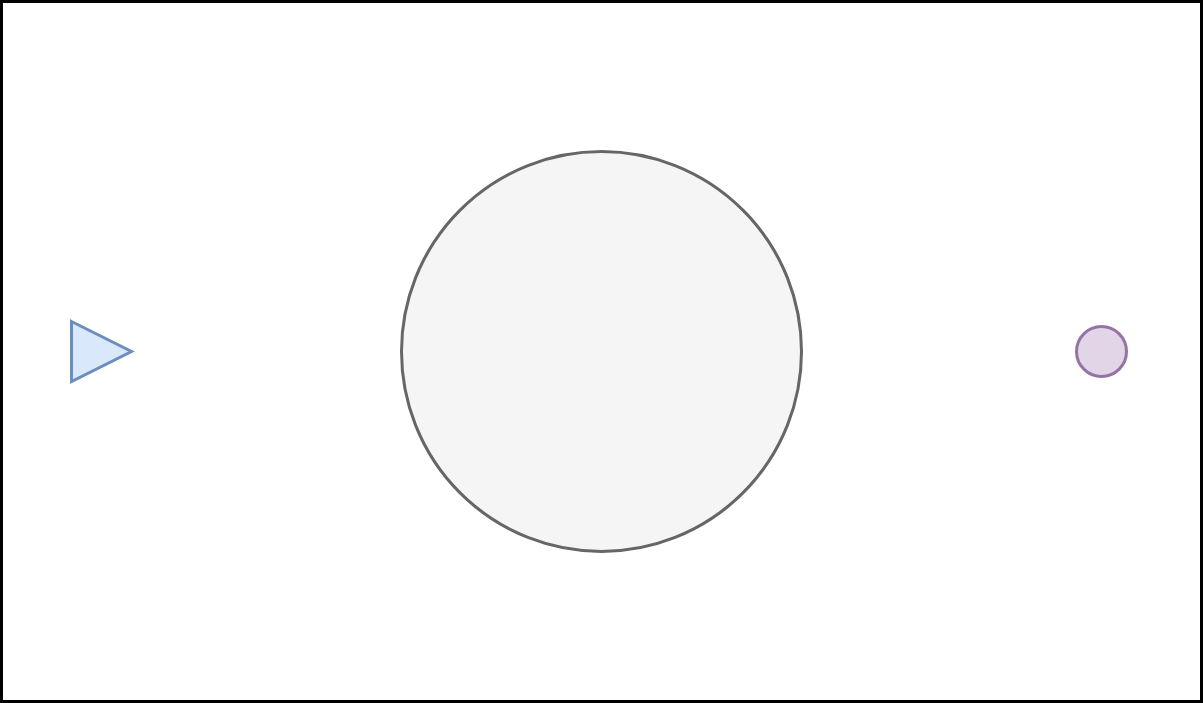
\includegraphics[width=\textwidth]{IMAGES/part3/map1.png}
		\caption*{Map 1}
		\label{fig:map1}
	\end{subfigure}
	\hfill
	\begin{subfigure}[b]{0.24\textwidth}
		\centering
		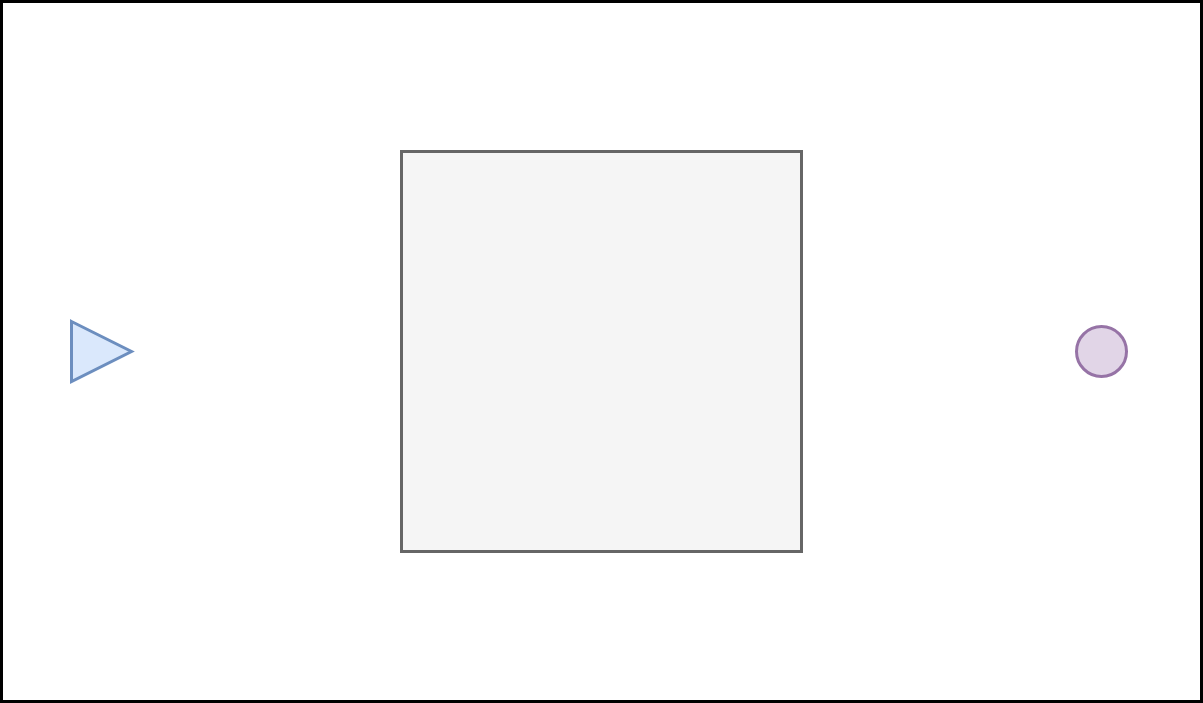
\includegraphics[width=\textwidth]{IMAGES/part3/map2.png}
		\caption*{Map 2}
		\label{fig:map2}
	\end{subfigure}
	\hfill
	\begin{subfigure}[b]{0.24\textwidth}
		\centering
		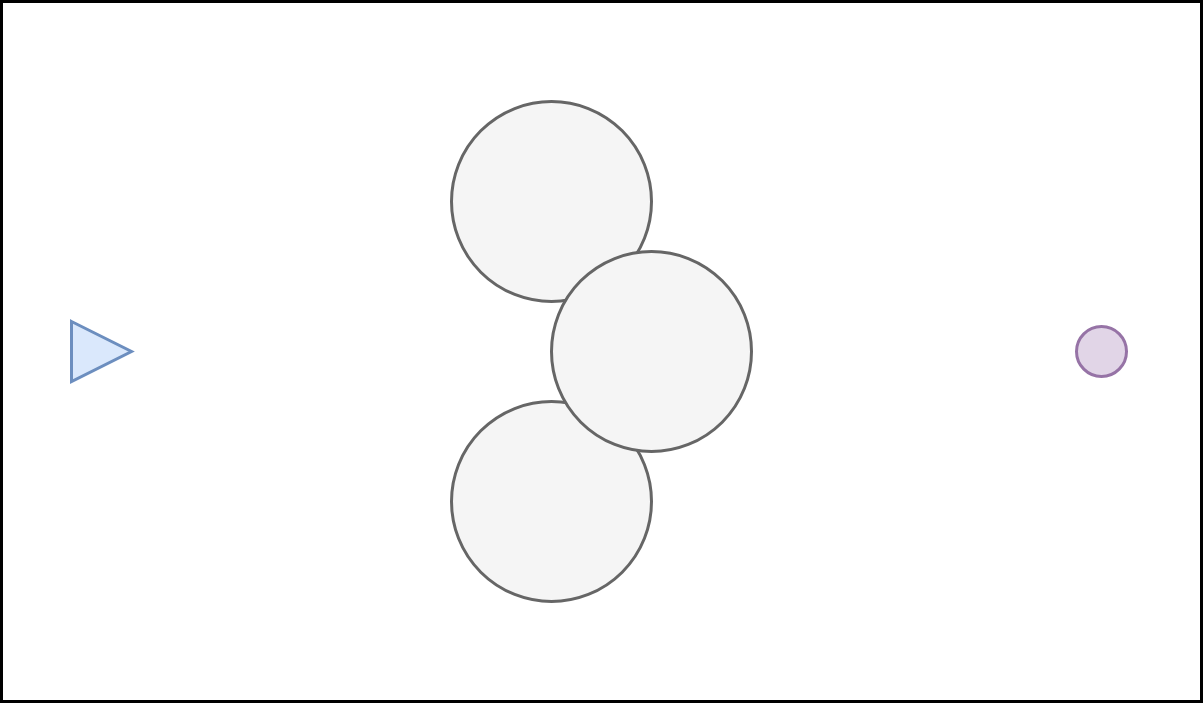
\includegraphics[width=\textwidth]{IMAGES/part3/map3.png}
		\caption*{Map 3}
		\label{fig:map3}
	\end{subfigure}
	\hfill
	\begin{subfigure}[b]{0.24\textwidth}
		\centering
		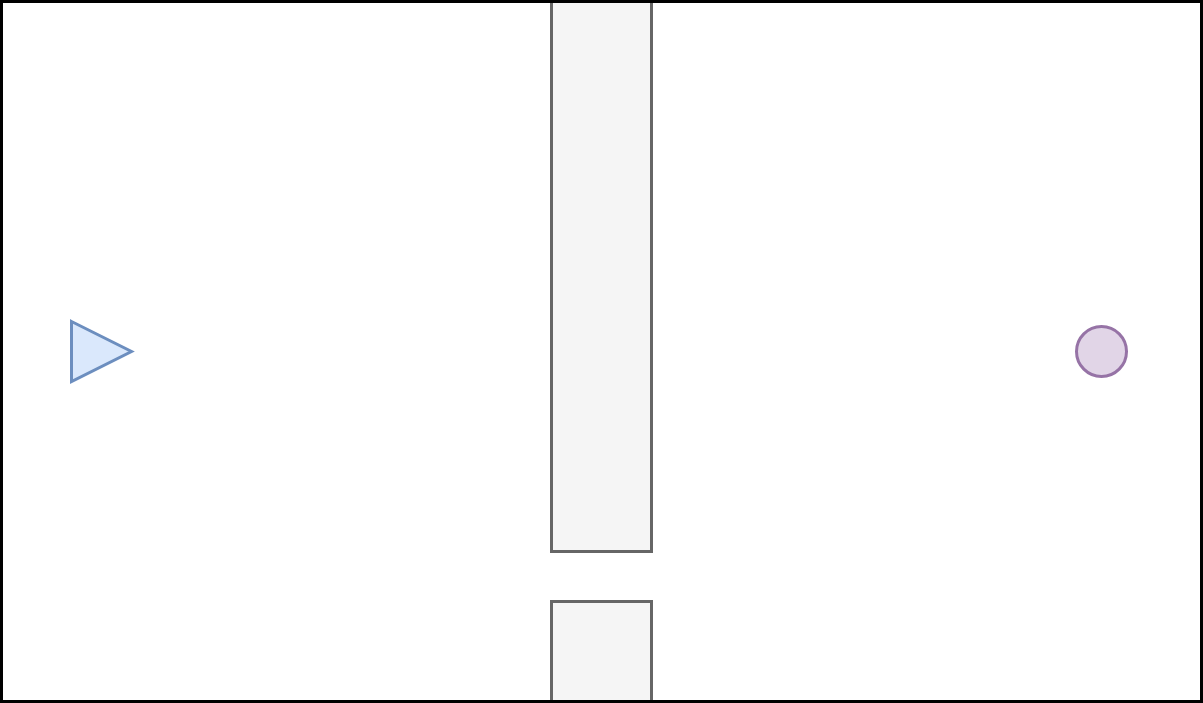
\includegraphics[width=\textwidth]{IMAGES/part3/map4.png}
		\caption*{Map 4}
		\label{fig:map4}
	\end{subfigure}
	\vfill
	\begin{subfigure}[b]{0.24\textwidth}
		\centering
		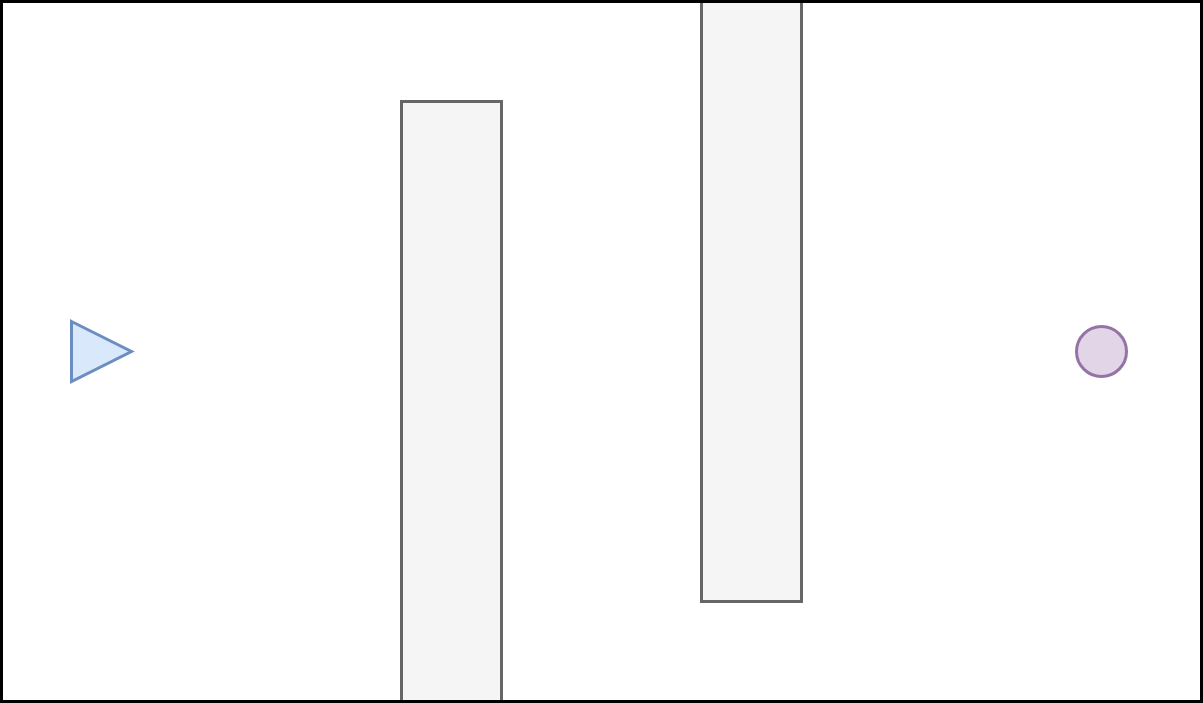
\includegraphics[width=\textwidth]{IMAGES/part3/map5.png}
		\caption*{Map 5}
		\label{fig:map5}
	\end{subfigure}
	\hfill
	\begin{subfigure}[b]{0.24\textwidth}
		\centering
		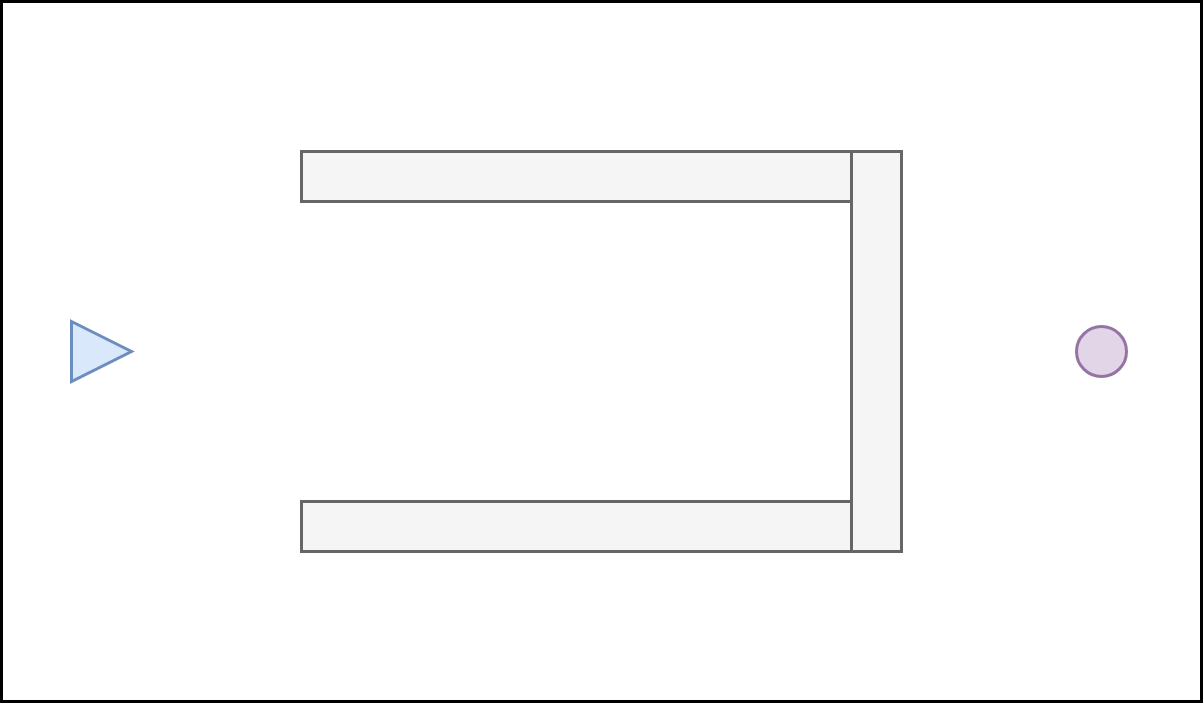
\includegraphics[width=\textwidth]{IMAGES/part3/map6.png}
		\caption*{Map 6}
		\label{fig:map6}
	\end{subfigure}
	\hfill
	\begin{subfigure}[b]{0.24\textwidth}
		\centering
		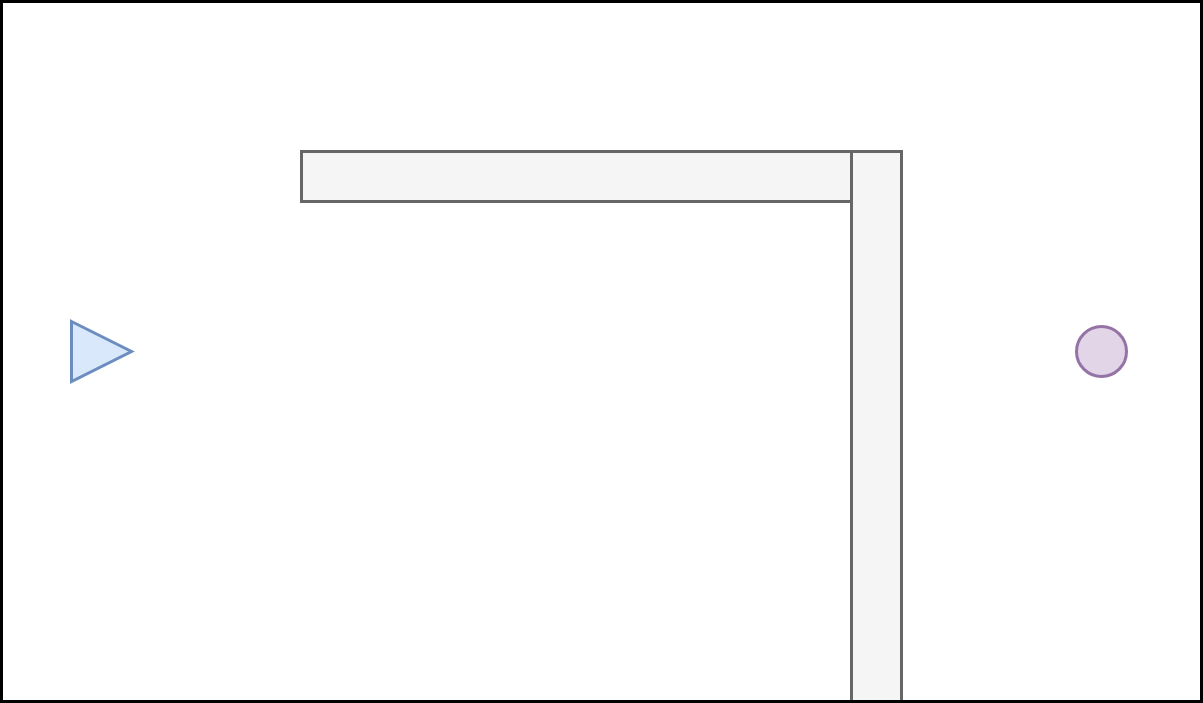
\includegraphics[width=\textwidth]{IMAGES/part3/map7.png}
		\caption*{Map 7}
		\label{fig:map7}
	\end{subfigure}
	\hfill
	\begin{subfigure}[b]{0.24\textwidth}
		\centering
		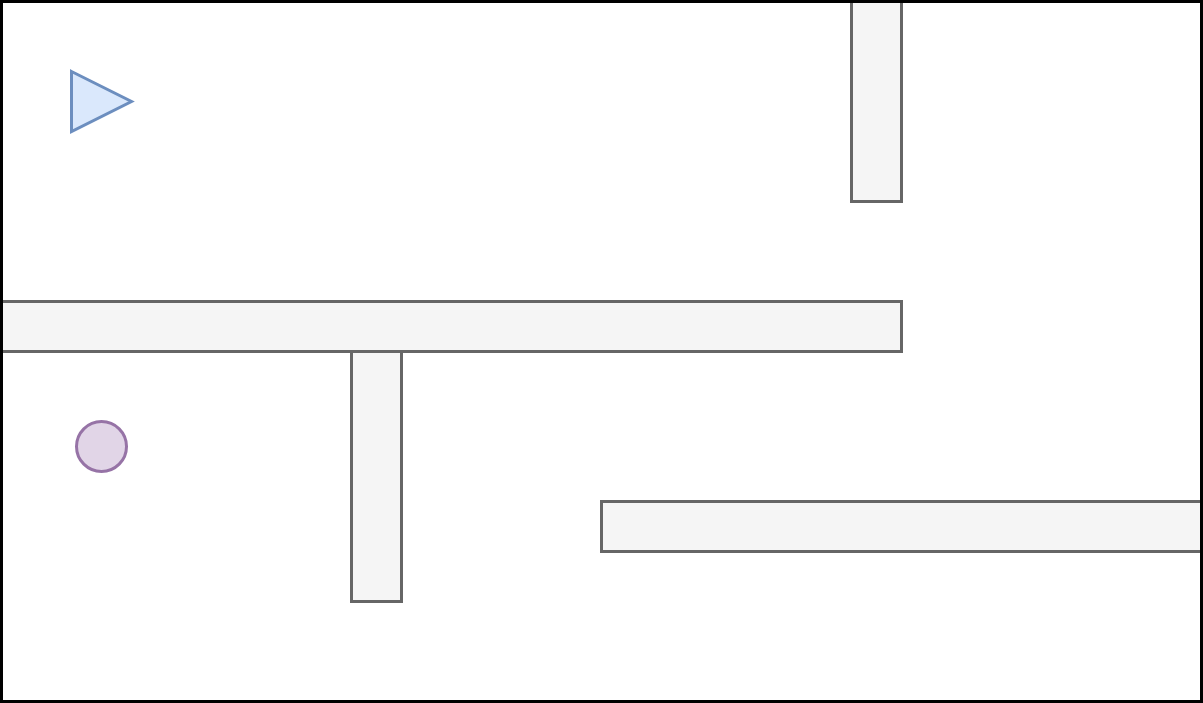
\includegraphics[width=\textwidth]{IMAGES/part3/map8.png}
		\caption*{Map 8}
		\label{fig:map8}
	\end{subfigure}
	\caption{Benchmark maps}
	\label{fig:benchmark_maps}
\end{figure}

\textbf{Results}
\begin{figure}[H]
	\centering
	\begin{subfigure}[b]{0.24\textwidth}
		\centering
		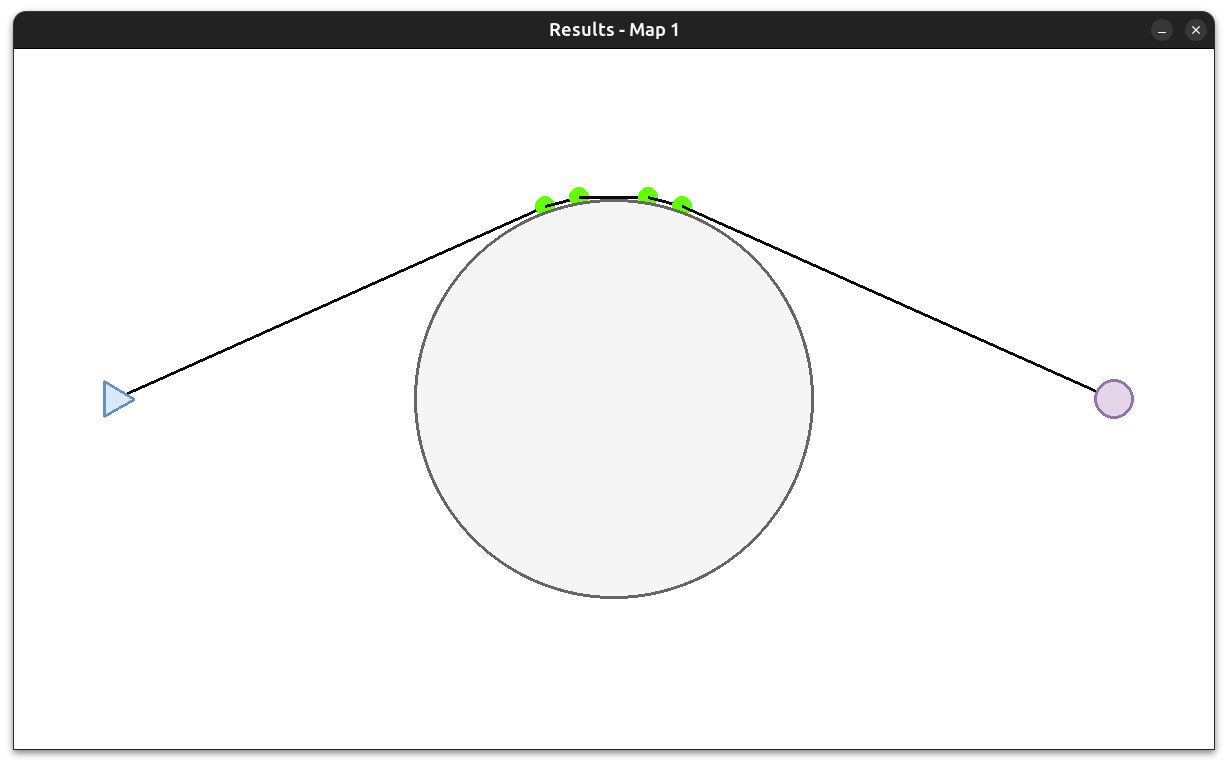
\includegraphics[width=\textwidth]{IMAGES/part3/rmap1.png}
		\caption*{Result for map 1}
		\label{fig:rmap1}
	\end{subfigure}
	\hfill
	\begin{subfigure}[b]{0.24\textwidth}
		\centering
		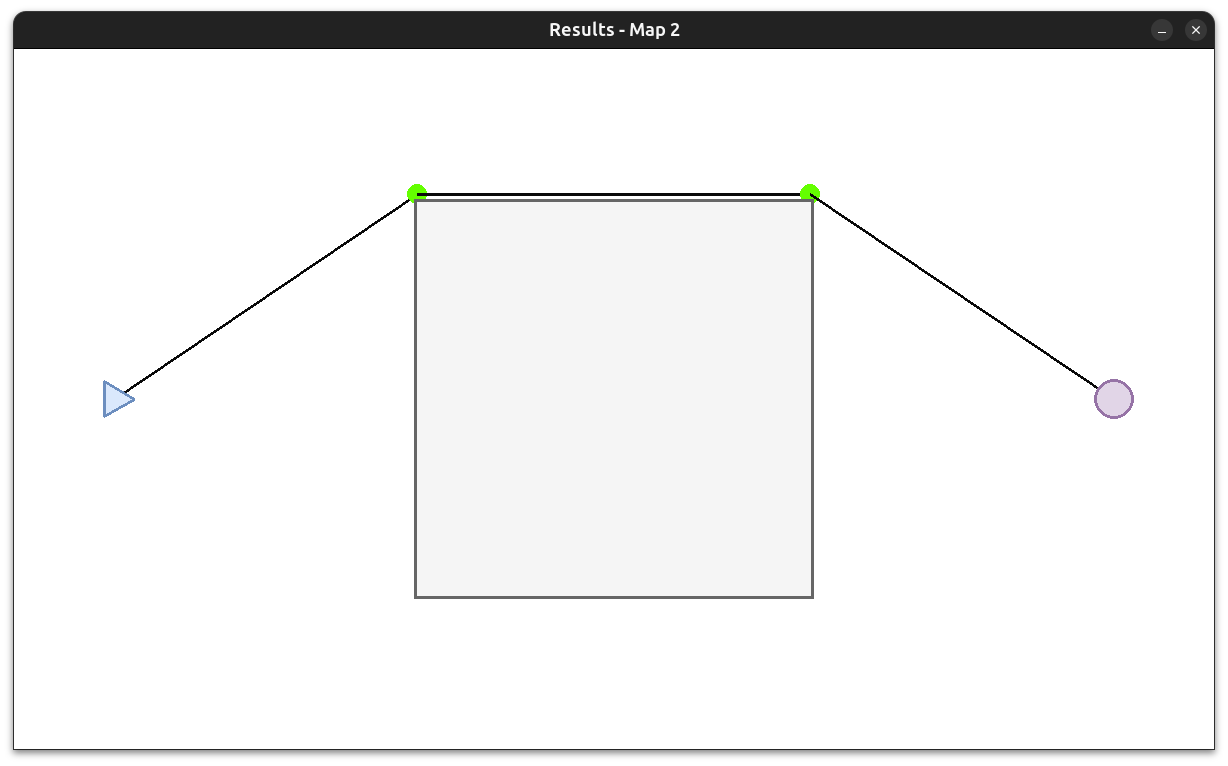
\includegraphics[width=\textwidth]{IMAGES/part3/rmap2.png}
		\caption*{Result for map 2}
		\label{fig:rmap2}
	\end{subfigure}
	\hfill
	\begin{subfigure}[b]{0.24\textwidth}
		\centering
		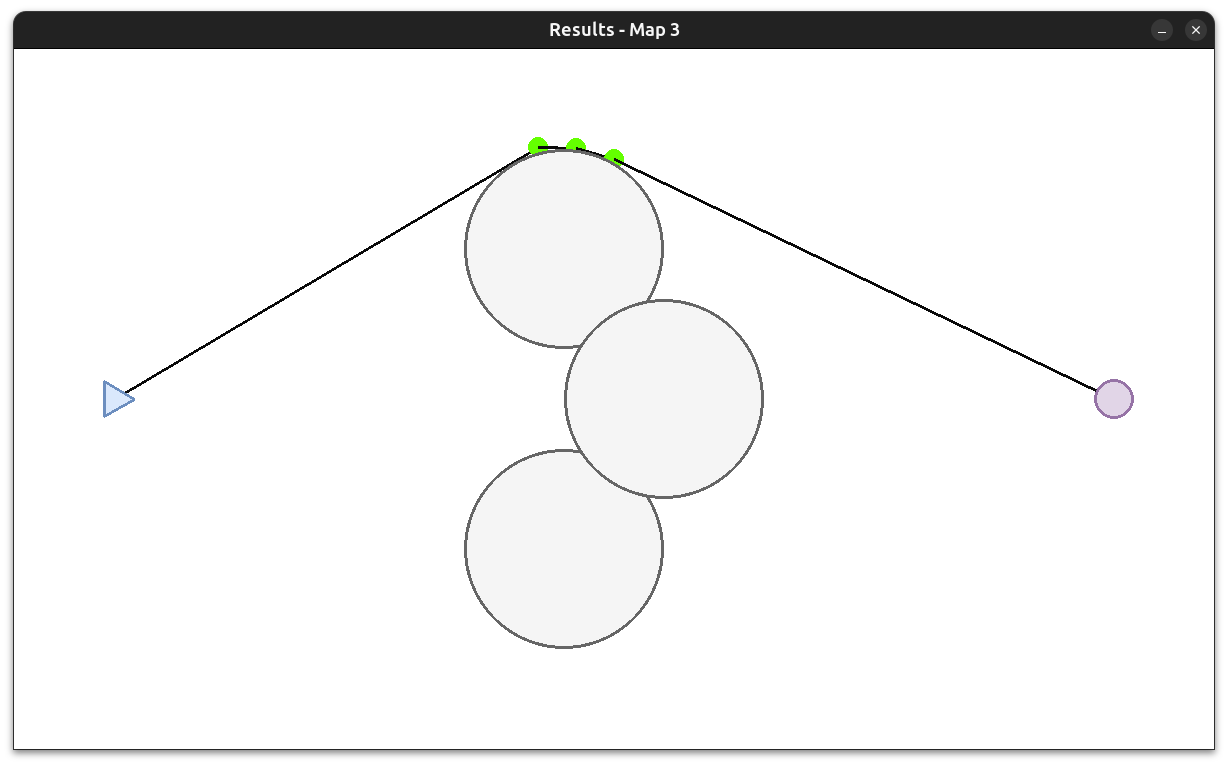
\includegraphics[width=\textwidth]{IMAGES/part3/rmap3.png}
		\caption*{Result for map 3}
		\label{fig:rmap3}
	\end{subfigure}
	\hfill
	\begin{subfigure}[b]{0.24\textwidth}
		\centering
		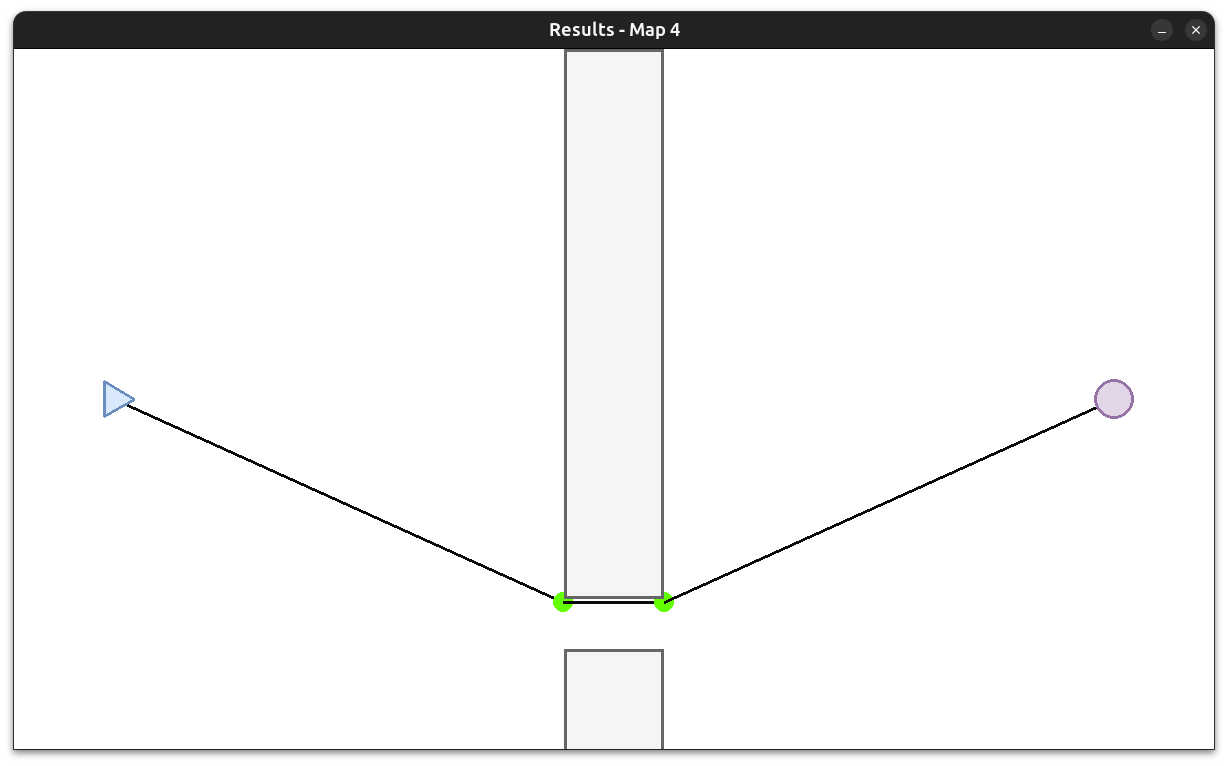
\includegraphics[width=\textwidth]{IMAGES/part3/rmap4.png}
		\caption*{Result for map 4}
		\label{fig:rmap4}
	\end{subfigure}
	\vfill
	\begin{subfigure}[b]{0.24\textwidth}
		\centering
		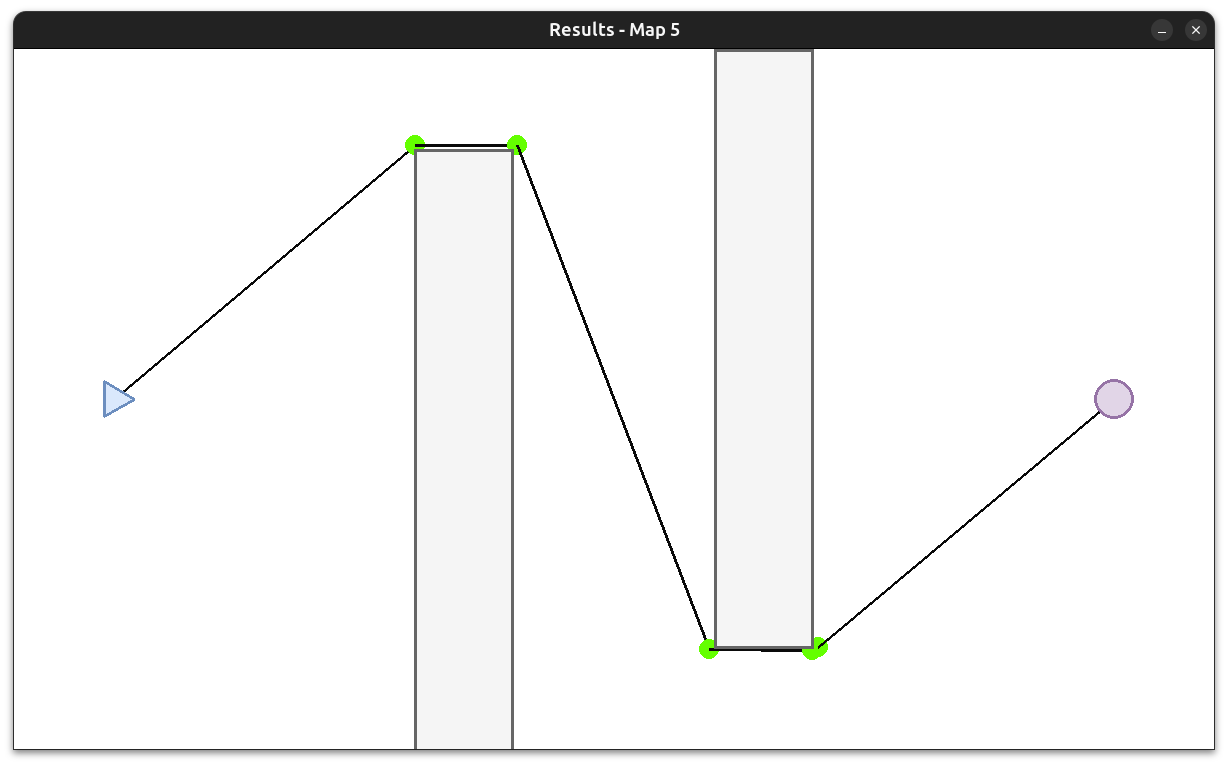
\includegraphics[width=\textwidth]{IMAGES/part3/rmap5.png}
		\caption*{Result for map 5}
		\label{fig:rmap5}
	\end{subfigure}
	\hfill
	\begin{subfigure}[b]{0.24\textwidth}
		\centering
		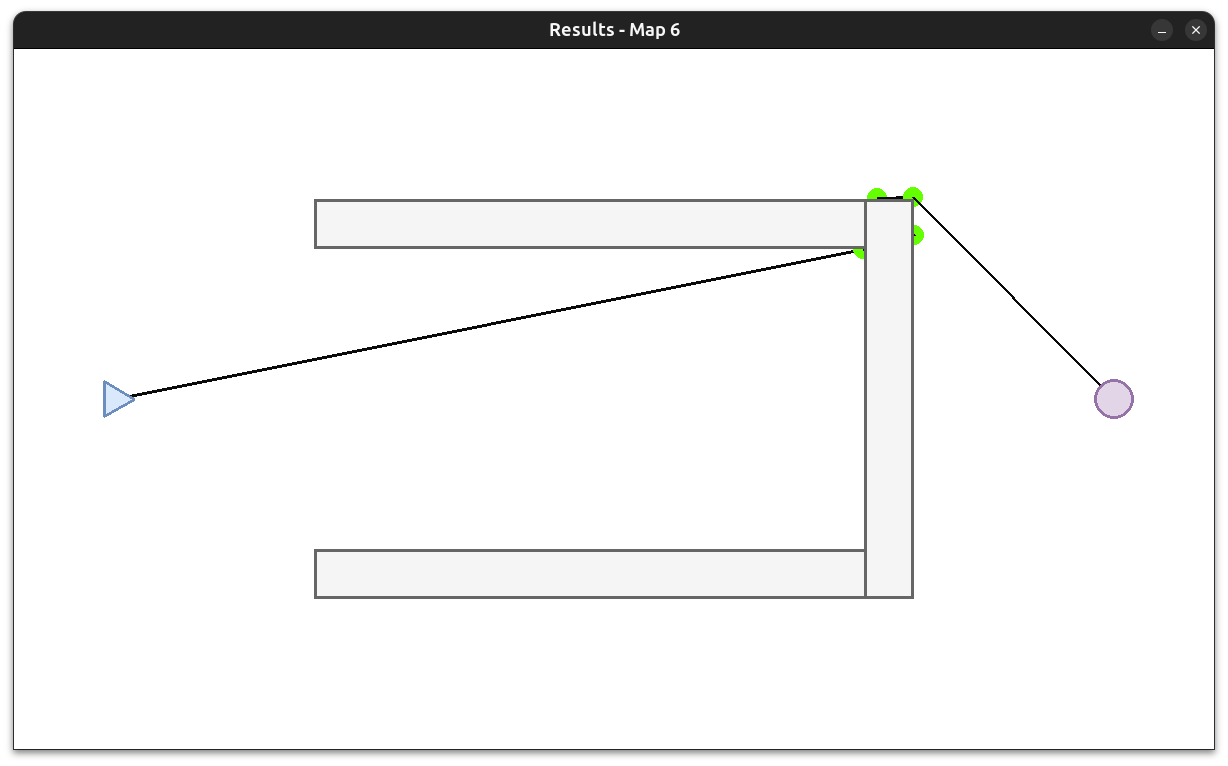
\includegraphics[width=\textwidth]{IMAGES/part3/rmap6.png}
		\caption*{Result for map 6}
		\label{fig:rmap6}
	\end{subfigure}
	\hfill
	\begin{subfigure}[b]{0.24\textwidth}
		\centering
		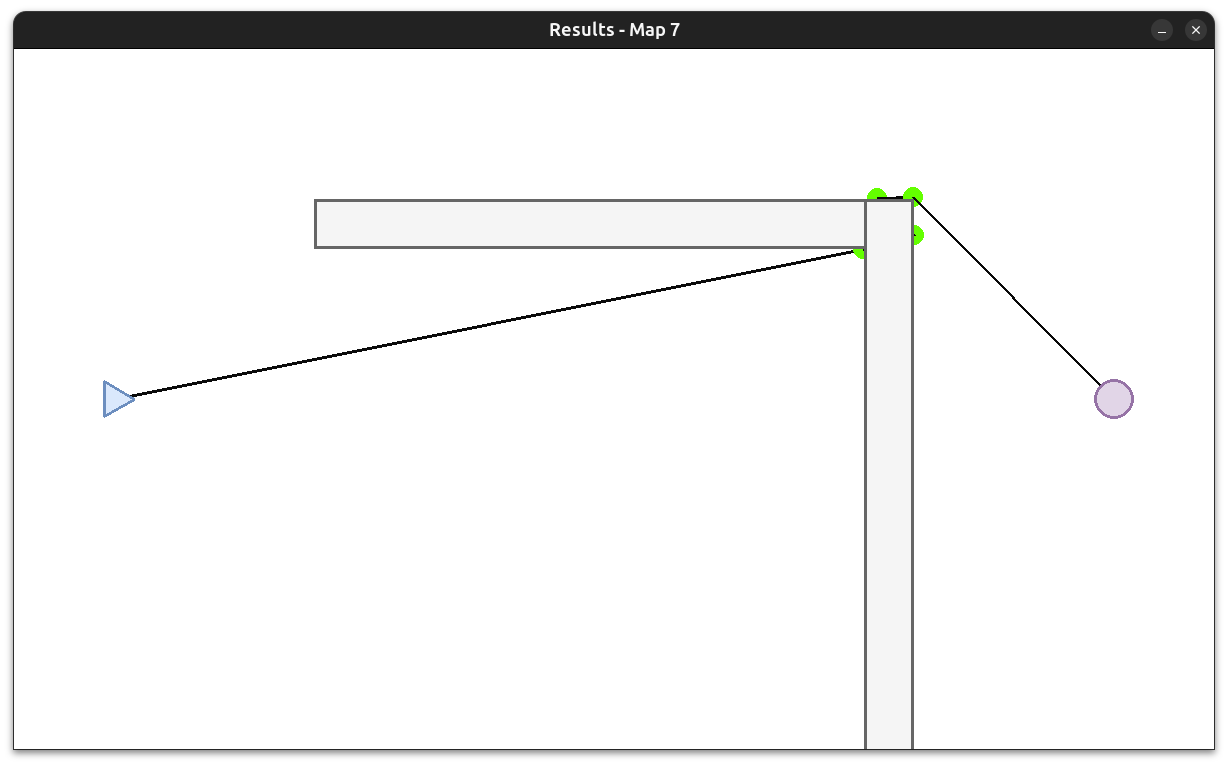
\includegraphics[width=\textwidth]{IMAGES/part3/rmap7.png}
		\caption*{Result for map 7}
		\label{fig:rmap7}
	\end{subfigure}
	\hfill
	\begin{subfigure}[b]{0.24\textwidth}
		\centering
		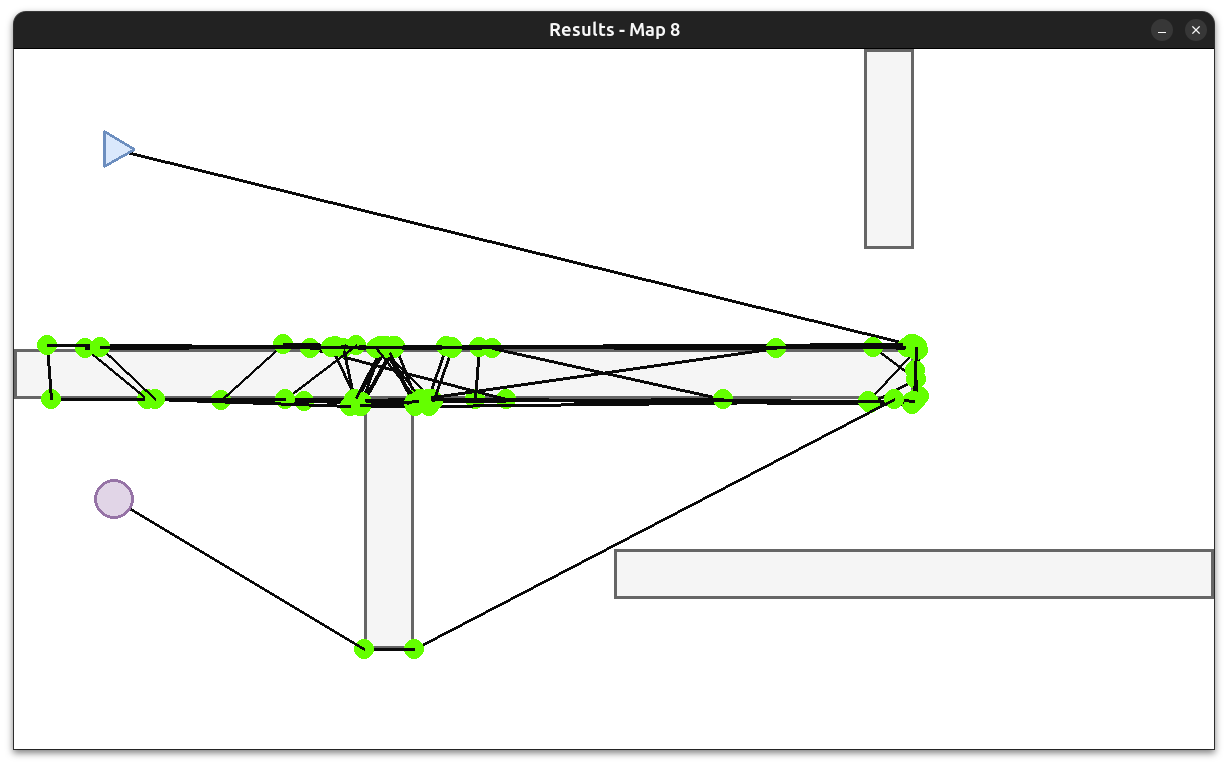
\includegraphics[width=\textwidth]{IMAGES/part3/rmap8.png}
		\caption*{Result for map 8}
		\label{fig:rmap8}
	\end{subfigure}
	\caption{Results on the benchmark maps}
	\label{fig:results_benchmark_maps}
\end{figure}


\textbf{Lenght of the path found in metric unit (mu)}
\begin{table}[H]
	\centering
	\begin{tabular}{c c c c}
		\hline
		Map & Theoretically & Method & Cellular Automata \\
		\hline
		Map 1 &  & 1084 &  \\
		Map 2 &  & 1125 & 1122 \\
		Map 3 &  & 1125 & 1122 \\
		Map 4 &  & 1088 & 1086 \\
		Map 5 &  & 1531 & 1522 \\
		Map 6 &  & - & 1168 \\
		Map 7 &  & - & 1168 \\
		Map 8 &  & - &  \\
		\hline
	\end{tabular}
	\caption{Benchmark results for the new method}
	\label{tab:benchmark_results}
\end{table}

\end{document}

